\documentclass[xcolor=table]{beamer}
\usepackage[utf8]{inputenc}
\usepackage{default}
\usepackage{rotating}
\usepackage{float}
\usepackage{tabularx}
\usepackage{multicol}
\usepackage{multirow}
\usepackage{adjustbox}
\usepackage{boldline}
\usepackage{amsmath}
\usepackage[table]{xcolor}

\newcommand\FourQuad[4]{%
 \begin{minipage}[b][.45\textheight][t] 
  {.48\textwidth}#1\end{minipage}\hfill%
 \begin{minipage}[b][.45\textheight][t] 
  {.48\textwidth}#2\end{minipage}\\[0.5em]
 \begin{minipage}[b][.45\textheight][t] 
  {.99\textwidth}#3\end{minipage}\hfill
 }
 
\newcommand\Quad[4]{%
 \begin{minipage}[b][.33\textheight][t] 
  {.48\textwidth}#1\end{minipage}\hfill%
 \begin{minipage}[b][.33\textheight][t] 
  {.48\textwidth}#2\end{minipage}\\[0.5em]
 \begin{minipage}[b][.33\textheight][t] 
  {.48\textwidth}#3\end{minipage}\hfill
 \begin{minipage}[b][.33\textheight][t] 
  {.48\textwidth}#4\end{minipage}%
 }
 
\usetheme{Madrid}

\title{Analysis of the Path Tracing rendering method on CPU and GPU}
\author{by Jordi Gil González}
\centering
\date{April 2020}
\begin{document}

\maketitle

\begin{frame}{Content}
	\begin{itemize}
		\item What is Path Tracing?
		\item Direct illumination vs. Global illumination
		\item Rendering Equation
		\item Anti-Aliasing
		\item Triangles
		\begin{itemize}
			\item Möller-Trumbore
		\end{itemize}
		\item Bounding Volume Hierarchy
		\begin{itemize}
			\item Ray-slab intersection
			\item LBVH - Tero Karras
		\end{itemize}
		\item Geometry transforms
		\item Materials
		\item Image Filters
		\item Results
	\end{itemize}
\end{frame}

\begin{frame}{What is Path Tracing?}

	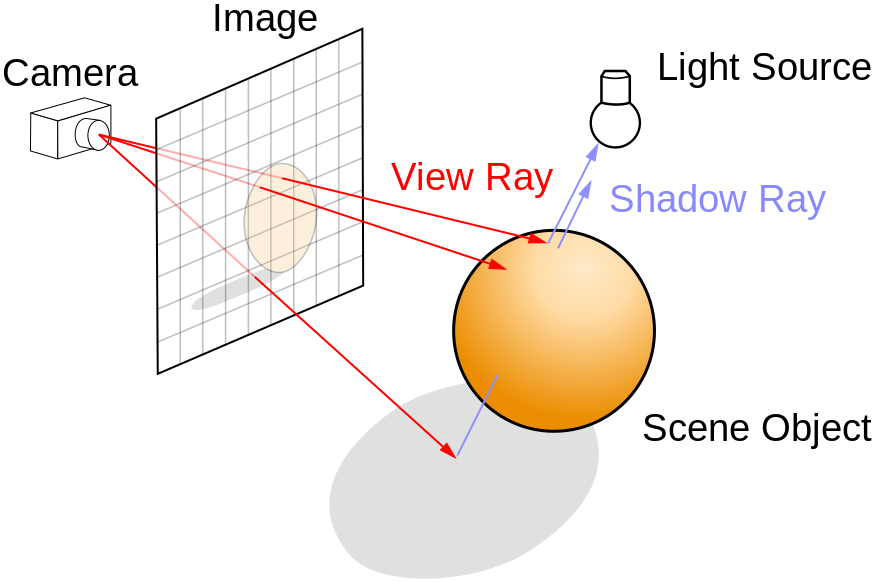
\includegraphics[scale=0.35]{media/Ray_trace_diagram.png}

\end{frame}

\begin{frame}{Direct illumination vs. Global illumination}

	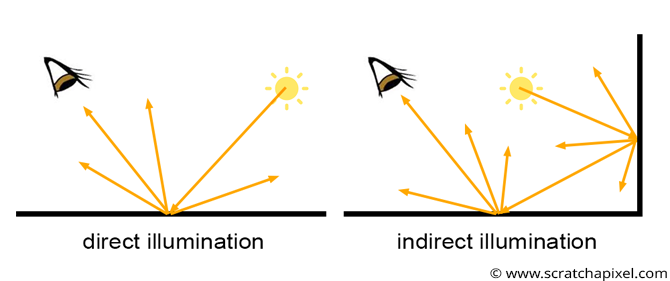
\includegraphics[scale=0.65]{media/shad2-globalillum3.png}

\end{frame}

\begin{frame}{Rendering Equation}

	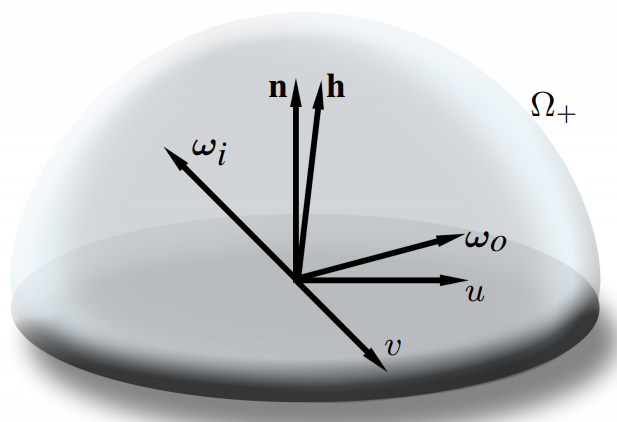
\includegraphics[scale=0.35]{media/Rendering_eq.png}
$$
L_o(x,\omega_o,\lambda,t) = L_e(x,\omega_o,\lambda,t) + L_r(x,\omega_i,\omega_o,\lambda,t)L_i(x,\omega_i,\lambda,t)
$$ 
\\
$$
L_o(x,\omega_o,\lambda,t) = L_e(x,\omega_o,\lambda,t) + \int_\Omega f_r(x,\omega_i,\omega_o,\lambda,t)L_i(x,\omega_i,\lambda,t)(\omega_i \cdot n) d\omega_i
$$

\end{frame}


\begin{frame}{Anti-aliasing}

\begin{itemize}
\item Supersampling
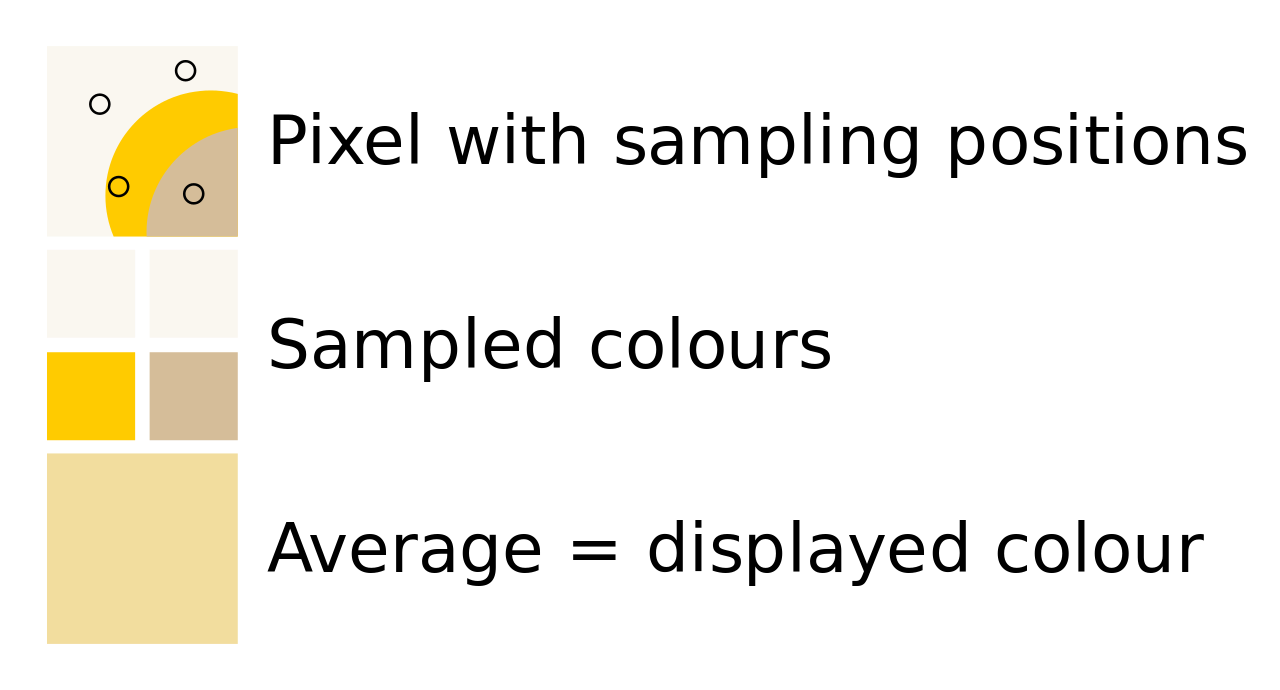
\includegraphics[scale=0.20]{media/Supersampling.png}
\end{itemize}

\end{frame}


\begin{frame}{Triangles}

	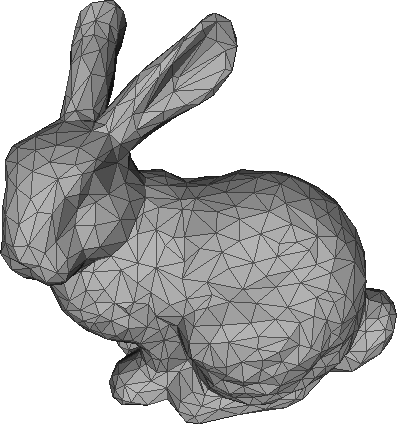
\includegraphics[scale=0.35]{media/snapshot00.png}

\end{frame}


\begin{frame}{Möller-Trumbore}
	$f(u,v) = p_0 + y \cdot p_1 + v \cdot p_2$, with $u \geq 0$, $v \geq 0$	and $u+v \leq 1$
	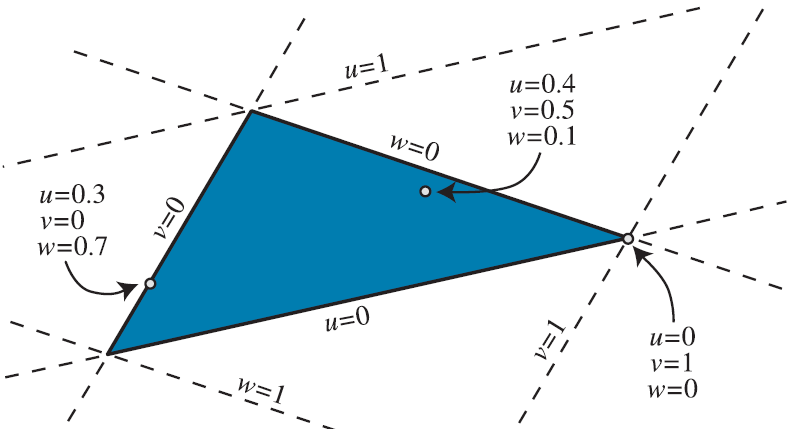
\includegraphics[scale=0.30]{media/barycentric.png}

\end{frame}

\begin{frame}{Möller-Trumbore}

	$\begin{bmatrix}
		-d & p_1 - p_0 & p_2 - p_0	
	\end{bmatrix}
	\begin{bmatrix}
	t \\ u \\ v
	\end{bmatrix}
	= o - p_o
	$
	
	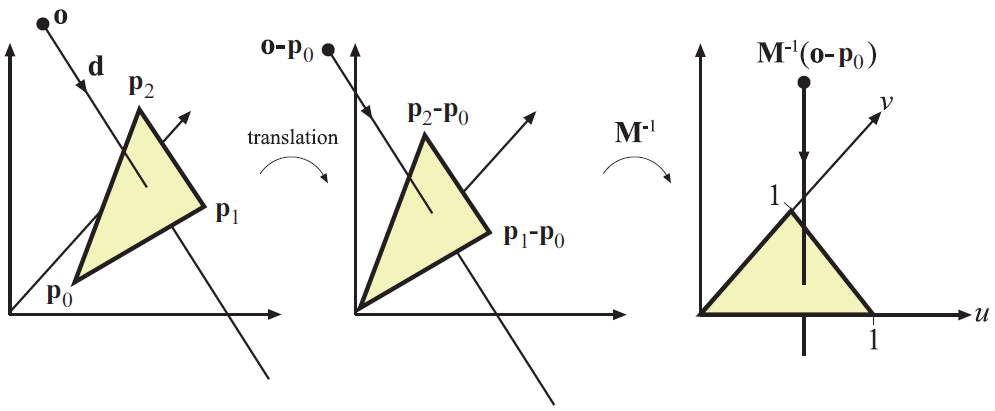
\includegraphics[scale=0.30]{media/transform.png}

\end{frame}

\begin{frame}{Bounding Volume Hierarchy I}

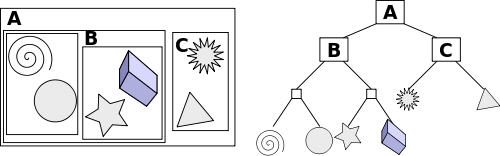
\includegraphics[scale=0.5]{media/BVH_example.png}

\end{frame}

\begin{frame}{Bounding Volume Hierarchy II}

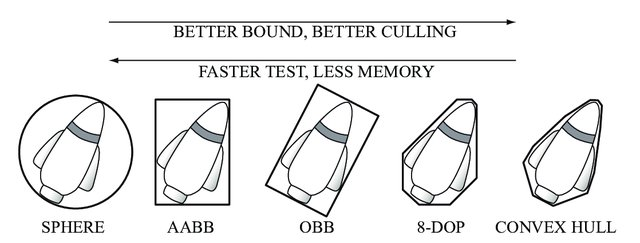
\includegraphics[scale=1.5]{media/volumes.jpg}

\end{frame}

\begin{frame}{Bounding Volume Hierarchy III}
\frametitle{Ray-slab intersection I}

\begin{columns}[T] % align columns

\begin{column}{.48\textwidth}

\begin{itemize}
\item Example with $t_{min}$. Same for $t_{max}$
\end{itemize}

$$
p_x + t_{x_{min}}d_x = x_{min}
$$
$$
t_{x_{min}} = \frac{\left( x_{min} - o_x\right)}{d_x}
$$
\\

$$
p_y + t_{y_{min}}d_y = y_{min}
$$
$$
t_{y_{min}} = \frac{\left( y_{min} - o_y\right)}{d_y}
$$
\end{column}%

\hfill%

\begin{column}{.48\textwidth}
\centering
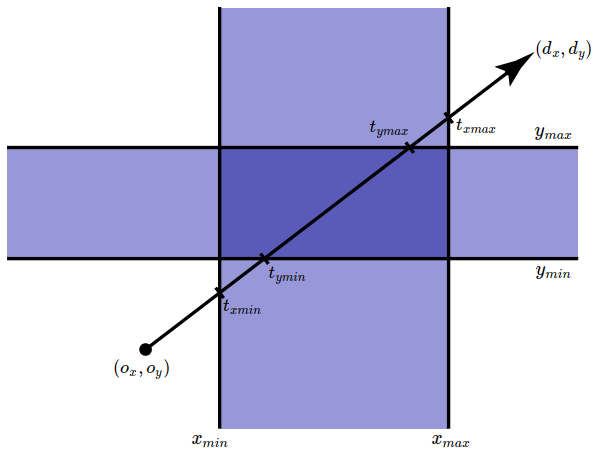
\includegraphics[scale=0.25]{media/slab_2.png}
$$
t_{min} = \left( \frac{\left( x_{min} - o_x\right)}{d_x}, \frac{\left( y_{min} - o_y\right)}{d_y} \right)
$$
\end{column}%

\end{columns}

\end{frame}

\begin{frame}{Ray-slab intersection II}

\begin{columns}[T] % align columns

\begin{column}{.48\textwidth}
\begin{itemize}
\item Each intersection is an interval
\item We want the last entry point $t_{smaller}$, and first exit point $t_{bigger}$
\end{itemize}

$$
t_{smaller} = min(t_{min}, t_{max})
$$
$$
t_{bigger} = max(t_{min}, t_{max})
$$
\begin{itemize}
\item $max(t_{x_{min}},t_{y_{min}},t_{z_{min}}) < min(t_{x_{max}},t_{y_{max}},t_{z_{max}})$
\end{itemize}
\end{column}%

\hfill%

\begin{column}{.48\textwidth}
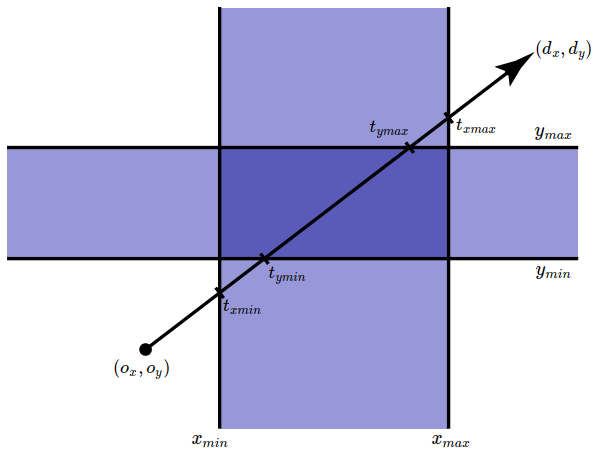
\includegraphics[scale=0.25]{media/slab_2.png}
\end{column}%

\end{columns}

\end{frame}

\begin{frame}{LBVH - Tero Karras}

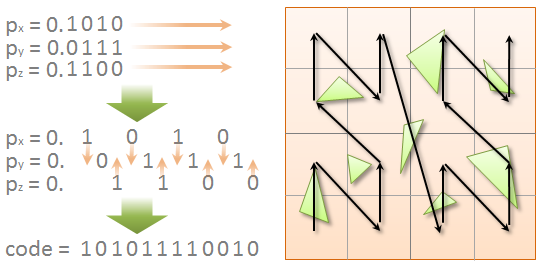
\includegraphics[scale=0.5]{media/fig04-z-curve.png}

\end{frame}

\begin{frame}{LBVH - Tero Karras}

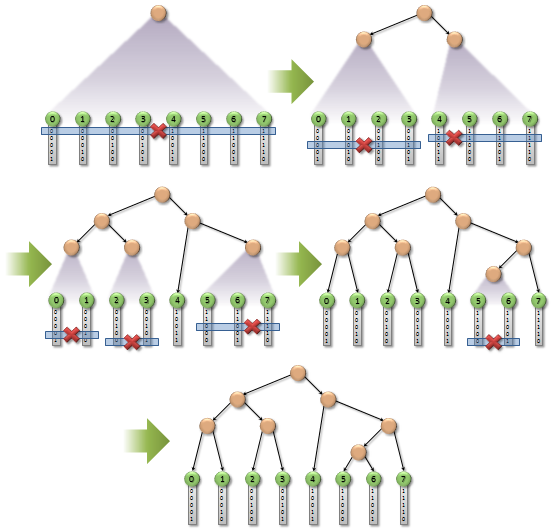
\includegraphics[scale=0.35]{media/fig05-top-down.png}

\end{frame}

\begin{frame}{Geometry Transforms}

\begin{itemize}
	\item Translation
	\item Scaling
	\item Rotation
\end{itemize}

\end{frame}

\begin{frame}{Translation}

\begin{itemize}
\item P in translated to P' by: \\
\centering
$
\begin{bmatrix}
1 & 0 & 0 & t_x \\
0 & 1 & 0 & t_y \\
0 & 0 & 1 & t_z \\
0 & 0 & 0 & 1 \\
\end{bmatrix}
\begin{bmatrix}
x \\ y \\ z \\ 1
\end{bmatrix}
=
\begin{bmatrix}
x' \\ y' \\ z' \\ 1
\end{bmatrix}
=
\begin{bmatrix}
x+t_x \\ y+t_y \\ z+t_z \\ 1
\end{bmatrix}
$
\end{itemize}
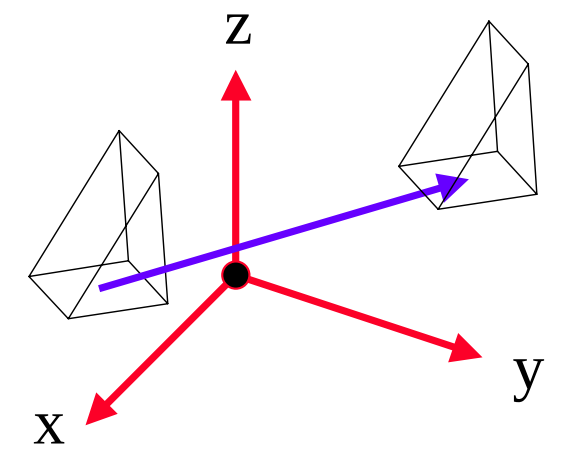
\includegraphics[scale=0.20]{media/translation.png}

\end{frame}

\begin{frame}{Scaling}

\centering
$
\begin{bmatrix}
s_x & 0 & 0 & 0 \\
0 & s_y & 0 & 0 \\
0 & 0 & s_z & 0 \\
0 & 0 & 0 & 1 \\
\end{bmatrix}
\begin{bmatrix}
x \\ y \\ z \\ 1
\end{bmatrix}
=
\begin{bmatrix}
x' \\ y' \\ z' \\ 1
\end{bmatrix}
=
\begin{bmatrix}
x s_x \\ y s_y \\ z s_z \\ 1
\end{bmatrix}
$
\\
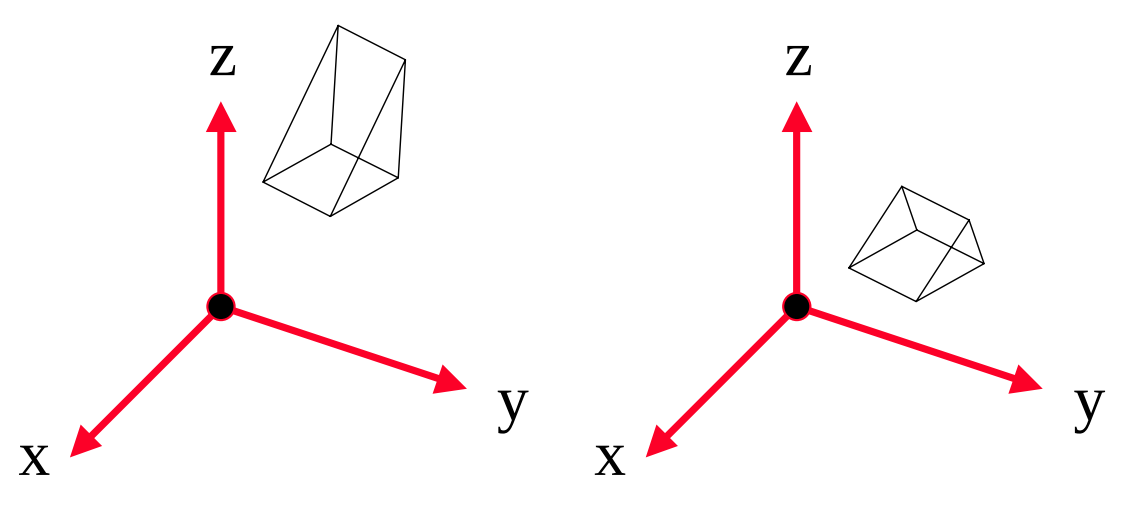
\includegraphics[scale=0.20]{media/scaling.png}

\end{frame}

\begin{frame}{Rotation}

\centering

\begin{align*}
\resizebox{\textwidth}{!}{$\displaystyle
R_x = 
\begin{bmatrix}
1 & 0 & 0 & 0 \\
0 & cos\theta_x & -sin\theta_x & 0 \\
0 & sin\theta_x & cos\theta_x & 0 \\
0 & 0 & 0 & 1 \\
\end{bmatrix}
R_y = 
\begin{bmatrix}
cos\theta_y & 0 & sin\theta_y & 0 \\
0 & 1 & 0 & 0 \\
-sin\theta_y  & 0 & cos\theta_y & 0 \\
0 & 0 & 0 & 1 \\
\end{bmatrix}
R_z = 
\begin{bmatrix}
cos\theta_z & \sin\theta_z & 0 & 0 \\
sin\theta_z & cos\theta_z & 0 & 0 \\
0 & 0 & 1 & 0 \\
0 & 0 & 0 & 1 \\
\end{bmatrix}
$}
\end{align*}

\begin{align*}
\resizebox{\textwidth}{!}{$\displaystyle
R = R_z \cdot R_y \cdot R_x =\begin{bmatrix}
cos\theta_y cos\theta_z 	& -cos\theta_x sin\theta_z + sin\theta_x sin\theta_y cos\theta_z & sin\theta_x sin\theta_z + cos\theta_x sin\theta_y cos\theta_z & 0 \\
cos\theta_y sin\theta_z 	& cos\theta_x cos\theta_z + sin\theta_x sin\theta_y sin\theta_z & -sin\theta_x cos\theta_z + cos\theta_x sin\theta_y sin\theta_z & 0 \\
-sin\theta_y 				& sin\theta_x cos\theta_y & cos\theta_x cos\theta_y & 0 \\
0 							& 0 & 0 & 1 \\
\end{bmatrix}
$}
\end{align*}
\\

\end{frame}

\begin{frame}{Materials I - Diffuse \& Metals}

\Quad%
   { 
   \begin{itemize}
   	\item<1-> Diffuse \\
   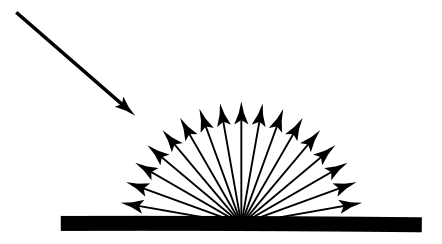
\includegraphics[scale=0.25]{media/Diffuse_Reflection.png}
   \end{itemize}
   }
   {
   \begin{itemize}
   	\item<1-> Metal \\
   	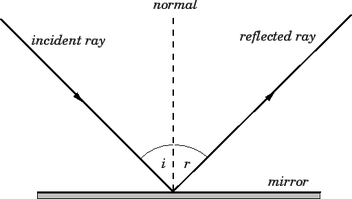
\includegraphics[scale=0.25]{media/reflection_ray.png}
   \end{itemize}
   }
   {
   	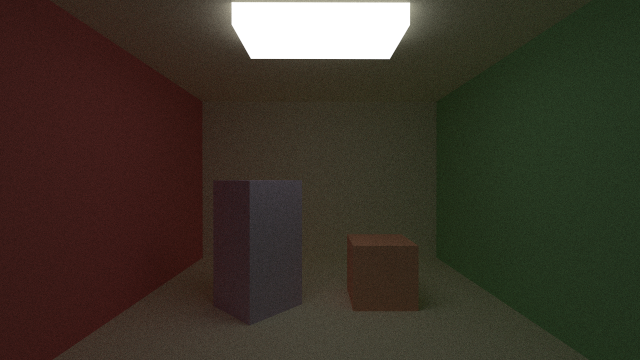
\includegraphics[scale=0.25]{media/cornell_normal_test.png}
   }
   {
   	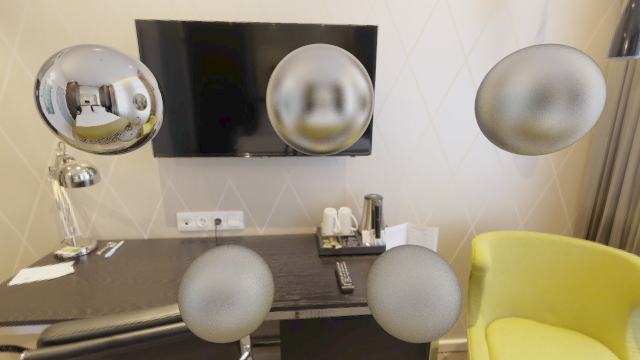
\includegraphics[scale=0.25]{media/example_metals.png}
   }

\end{frame}

\begin{frame}{Materials II - Dielectrics \& Textures}

\Quad%
   { 
   \begin{itemize}
   	\item<1-> Dielectrics \\
   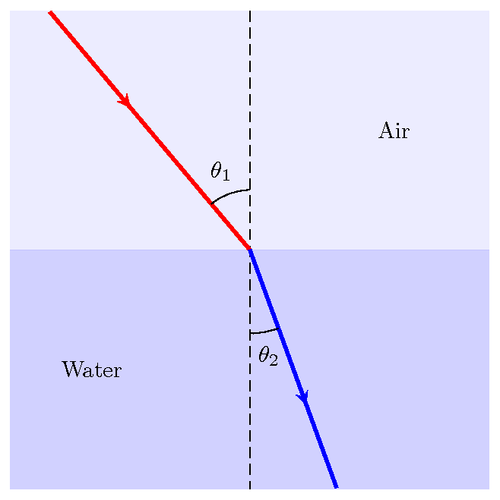
\includegraphics[scale=0.15]{media/refraction.png}
   \end{itemize}
   }
   {
   \begin{itemize}
   	\item<1-> Textures \\
   	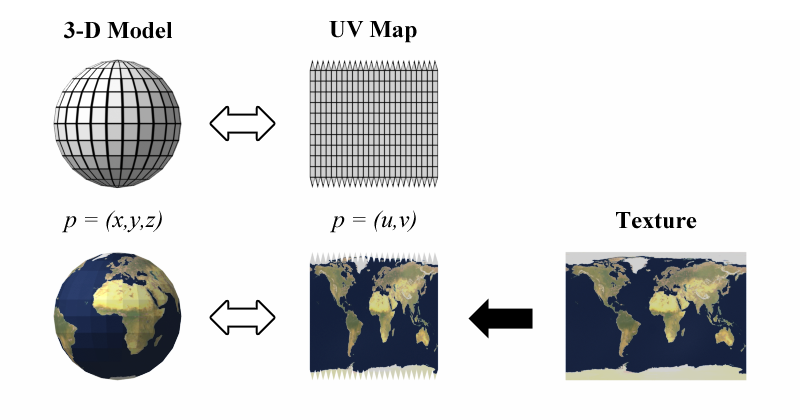
\includegraphics[scale=0.15]{media/UVMapping.png}
   \end{itemize}
   }
   {
   \centering
   	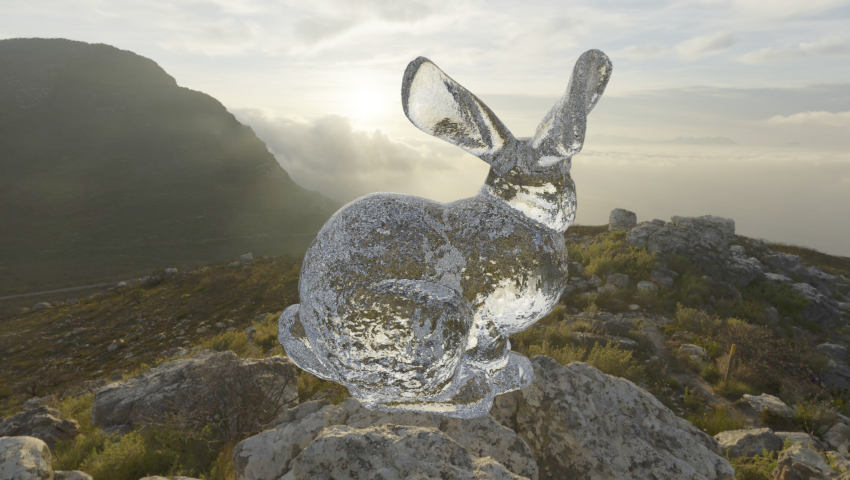
\includegraphics[scale=0.185]{media/CapeHill_cristal_bunny_2.png}
   }
   {
   	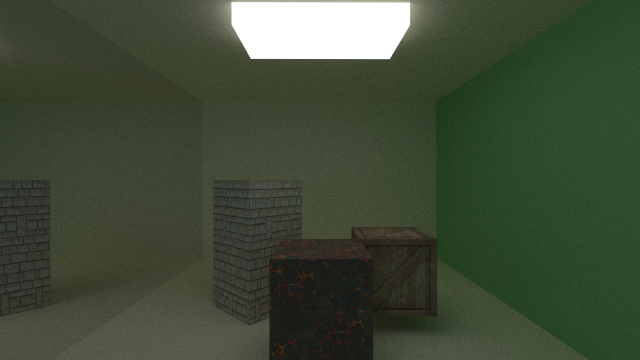
\includegraphics[scale=0.25]{media/cornell_textures.png}
   }

\end{frame}

\begin{frame}{Materials III - Skybox}
\centering
\begin{columns}[T] % align columns
	\begin{column}{.48\textwidth}
		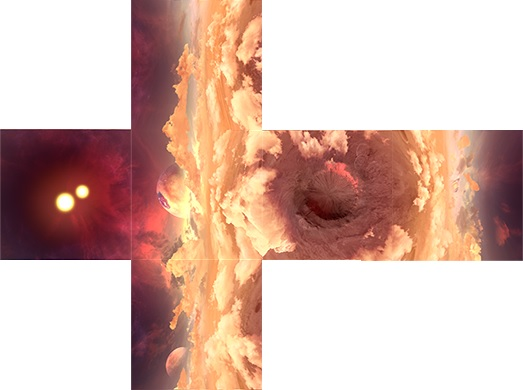
\includegraphics[scale=0.30]{media/cubemap-cross.jpg}
	\end{column}%
	\hfill%
	\begin{column}{.48\textwidth}
		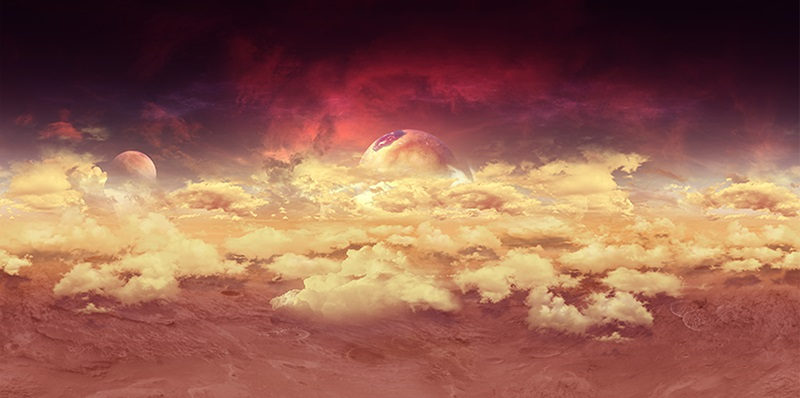
\includegraphics[scale=0.20]{media/skybox-assembled.jpg}
	\end{column}%
\end{columns}

\end{frame}


\begin{frame}{Image Filters}
  \FourQuad%
   { 
   \begin{itemize}
   	\item<1-> Mean Filter \\
   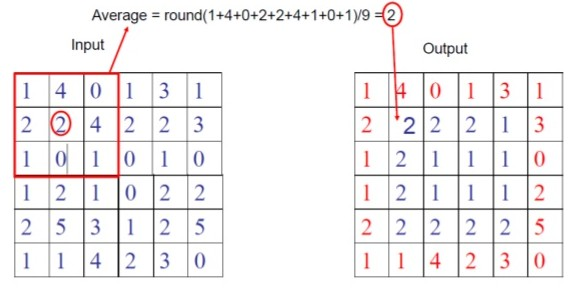
\includegraphics[scale=0.25]{media/noise-filtering-49-638.jpg}
   \end{itemize}
   }
   {
   \begin{itemize}
   	\item<1-> Median Filter \\
   	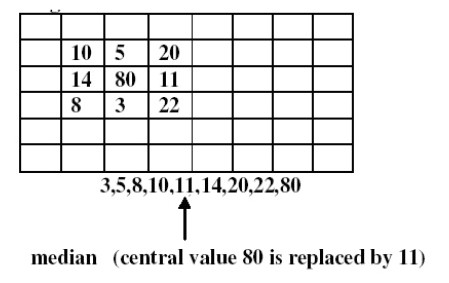
\includegraphics[scale=0.25]{media/median.jpg}
   \end{itemize}
   }
   {
   \begin{itemize}
   	\item<1-> Bilateral Filter \\
   	\centering
   	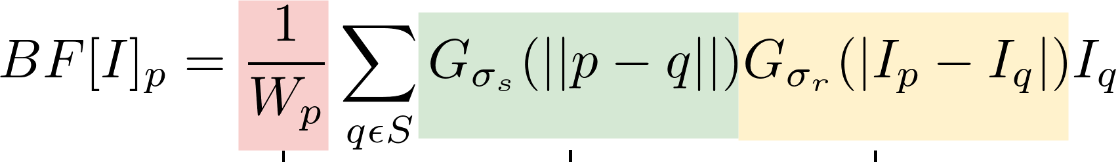
\includegraphics[scale=0.25]{media/Untitled-Diagram-138.png}
   \end{itemize}
   }
   
\end{frame}

\begin{frame}{Results}
  \FourQuad%
   { 
   \centering
   	\begin{figure}
   	\caption{Scene one}   	
   	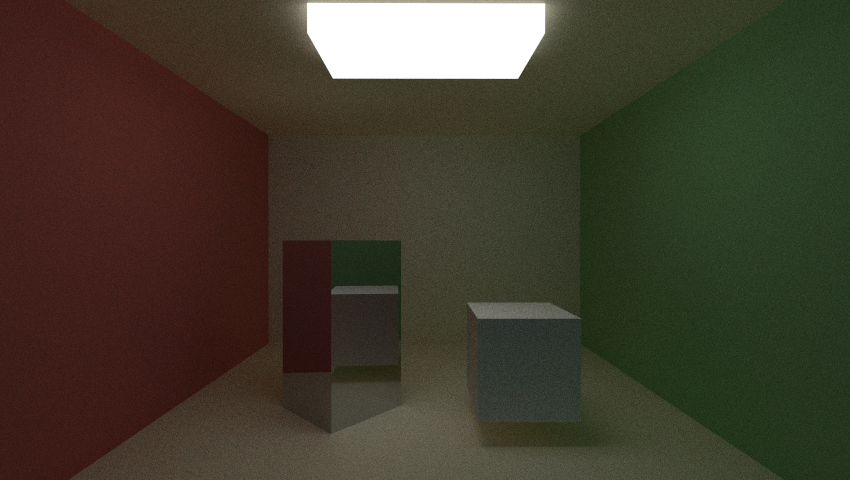
\includegraphics[scale=0.16]{media/cornell_normal.png}
   	\end{figure}
   }
   { 
   \centering
   	\begin{figure}
   	\caption{Scene two}  
   	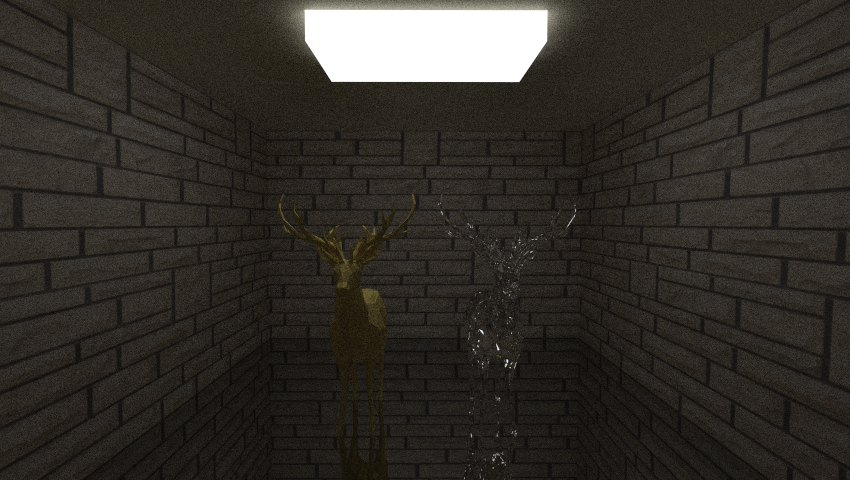
\includegraphics[scale=0.16]{media/cornell_deer_textures.png} 	
   	\end{figure}
   }
   {
   \centering
   	\begin{figure}
   	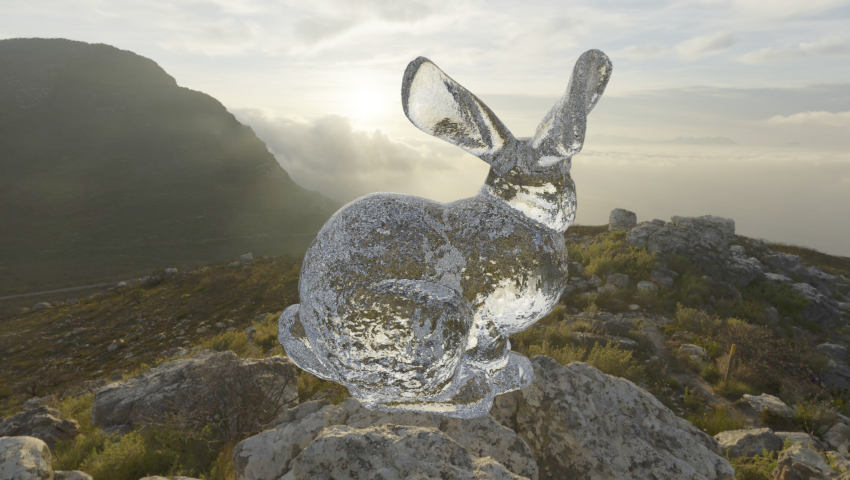
\includegraphics[scale=0.16]{media/CapeHill_cristal_bunny_2.png}
   	\caption{Scene three}   	
   	\end{figure}
   }

\end{frame}

\begin{frame}{Scene one}
\setlength\tabcolsep{10pt}
\resizebox{\textwidth}{!}{%
\begin{tabular}{*{9}{|c}|}
\hline
         \multicolumn{3}{|c|}{\multirow{2}{*}{Version}} & \multirow{2}{*}{Machine} & \multicolumn{5}{|c|}{Scene one} \\
         \multicolumn{3}{|c|}{} &  & \multicolumn{5}{|c|}{Time (\textit{seconds})}  \\ \hline
         & & & & 1 sample(s) & 10 sample(s) & 50 sample(s) & 100 sample(s) & 200 sample(s) \\ \hlineB{3.5}
         \multirow{12}*{CPU} & \multirow{6}*{Seq.}  & 
         	\multirow{2}*{List} & 
         		Lenovo 	& 15,50 & 154,14 & 774,44 & 1542,36 & 3095,65 \\ \cline{4-9}
         	& & &
         		Desktop & 14,12 & 139,79 & 742,83 & 1445,64 & 2809,16 \\ \clineB{3-9}{3.5}
		 & &        	
         	\multirow{2}*{BVH It.} &
         		Lenovo 	& 30,85 & 300,05 & 1493,99 & 3045,05 & 6081,05 \\ \cline{4-9}
         	& & &
         		Desktop & 27,51 & 273,01 & 1369,04 & 2729,36 & 5462,02 \\ \clineB{3-9}{3.5}
         & &        	
         	\multirow{2}*{BVH Rec.} &
         		Lenovo 	& 28,22 & 282,373 & 1407,27 & 2815,23 & 5632,42 \\ \cline{4-9}
         	& & &
         		Desktop & 26,06 & 258,99 & 1285,07 & 2568,13 & 5156,55  \\ \clineB{2-9}{3.5}
         		
         & \multirow{6}*{\texttt{OpenMP}}  &
         	\multirow{2}*{List} & 
         		Lenovo 	& 9,54 & 94,16 & 480,20 & 982,87 & 1929,72 \\ \cline{4-9}
         	& & &
         		Desktop & 8,79 & 88,81 & 460,89 & 877,24 & 1859,07 \\ \clineB{3-9}{3.5}
		 & &        	
         	\multirow{2}*{BVH It.} &
         		Lenovo 	&  10,08 & 102,17 & 525,59 & 1194,84 & 2159,8\\ \cline{4-9}
         	& & &
         		Desktop & \cellcolor{blue!25}9,01 & 90,48 & 451,49 & 916,96 & 1801,08\\ \clineB{3-9}{3.5}
         & &        	
         	\multirow{2}*{BVH Rec.} &
         		Lenovo 			& 11,40 & 122,50 	& 601,731 	& 1169,89 	& 2033,67  \\ \cline{4-9}
         	& & &
         		Desktop 		& 9,24 	& 88,62 	& 449,78 	& 896,47 	& 1762,38  \\ \clineB{1-9}{3.5}
         		
         \multirow{18}*{GPU} & \multirow{18}*{\texttt{CUDA}} &
         	\multirow{6}*{List} & 
         		Lenovo 			& 2,58 	& 25,76 & 128,43 	& 257,42	& 513,87	\\ \cline{4-9}
         	& & &
         		Desktop 		& 0,93 	& 9,38 	& \cellcolor{red!25}46,57 	& 91,85 	& 187,2    	\\ \cline{4-9}
         	& & &
         		BOADA - 1 GPU(s) 	& 3,13  & 27,53 & 135,83  	& 271,39 	& -   		\\ \cline{4-9}
         	& & &
         		BOADA - 2 GPU(s) 	& 2,07 	& 14,88 & 71,67 	& 142,867 	& 285,18   	\\ \cline{4-9}
         	& & &
         		BOADA - 3 GPU(s) 	& 1,87 	& 10,58 & \cellcolor{red!25}49,32 	& 97,80 	& 194,22   	\\ \cline{4-9}
         	& & &
         		BOADA - 4 GPU(s) 	& 1,83 	& 8,45 	& 37,77 	& 74,38 	& 147,36 	\\ \clineB{3-9}{3.5}
		 & &        	
         	\multirow{6}*{BVH It.} &
         		Lenovo 	& 5,68 & 56,58 & \cellcolor{red!25}285,36 &  1138,34  & 1703,40  \\ \cline{4-9}
         	& & &
         		Desktop & 1,495 & 15,11 & \cellcolor{red!25}75,14 & 149,00 & 300,13 \\ \cline{4-9}
         	& & &
         		BOADA - 1 GPU(s) & \cellcolor{blue!25}4,46 & 45,66 & 226,37 &  452,18 & -   \\ \cline{4-9}
         	& & &
         		BOADA - 2 GPU(s) & 3,05 & 24,26 & 118,67 &  236,20 &  - \\ \cline{4-9}
         	& & &
         		BOADA - 3 GPU(s) & 2,53 & 16,66 & \cellcolor{red!25}79,75 & 158,22 & 316,99 \\ \cline{4-9}
         	& & &
         		BOADA - 4 GPU(s) & 2,40 & 13,17  & 61,34 & 120,84  & 240,43 \\ \clineB{3-9}{3.5}
         & &        	
         	\multirow{6}*{BVH Rec.} &
         		Lenovo 	& 6,09 & 60,79 & 304,07 & 608,53 & 1216,93  \\ \cline{4-9}
         	& & &
         		Desktop &  9,09 & 108,15 & 557,74 & 1092,76 & -   \\ \cline{4-9}
         	& & &
         		BOADA - 1 GPU(s) & \cellcolor{blue!25}21,64 & 212,176 & - &  - & -   \\ \cline{4-9}
         	& & &
         		BOADA - 2 GPU(s) & 11,83 & 111,84 & 555,42 & - & - \\ \cline{4-9}
         	& & &
         		BOADA - 3 GPU(s) & 8,51 & 75,54 & 375,68 & - & - \\ \cline{4-9}
         	& & &
         		BOADA - 4 GPU(s) & 6,99 & 57,98 & 284,42 & - & - \\ \clineB{1-9}{5}
\end{tabular}}
\end{frame}

\begin{frame}{Scene two}
\setlength\tabcolsep{10pt}
\resizebox{\textwidth}{!}{%
\begin{tabular}{*{9}{|c}|}
         \hline
         \multicolumn{3}{|c|}{\multirow{2}{*}{Version}} & \multirow{2}{*}{Machine} & \multicolumn{5}{|c|}{Scene two} \\
         \multicolumn{3}{|c|}{} &  & \multicolumn{5}{|c|}{Time (\textit{seconds})}  \\ \hline
         & & & & 1 sample(s) & 10 sample(s) & 50 sample(s) & 100 sample(s) & 200 sample(s) \\ \hlineB{3.5}
         \multirow{12}*{CPU} & \multirow{6}*{Seq.}  & 
         	\multirow{2}*{List} & 
         		Lenovo 			& 997,50 & 9945,55 & - & - & -  \\ \cline{4-9}
         	& & &
         		Desktop 		& 895,25 & 8947,03 & - & - & - \\ \clineB{3-9}{3.5}
		 & &        	
         	\multirow{2}*{BVH It.} &
         		Lenovo 			& 63,40 & & & & \\ \cline{4-9}
         	& & &
         		Desktop		 	& 54,94 & 549,40 & 2752,72 & - & - \\ \clineB{3-9}{3.5}
         & &        	
         	\multirow{2}*{BVH Rec.} &
         		Lenovo 			& 61,14 & 574,35 & 2879,1 & - & -   \\ \cline{4-9}
         	& & &
         		Desktop 		& 52,63 & 517,39 & 2590,70 & - & - \\ \clineB{2-9}{3.5}
         		
         & \multirow{6}*{\texttt{OpenMP}}  &
         	\multirow{2}*{List} & 
         		Lenovo 			& 200,01 & 2049,1 & - & - & -  \\ \cline{4-9}
         	& & &
         		Desktop 		& 162,58 & 1628,67 & - & - & - \\ \clineB{3-9}{3.5}
		 & &        	
         	\multirow{2}*{BVH It.} &
         		Lenovo 			& 15,98 & 186,40 & 830,45 & 1603,2 & 3725,69	\\ \cline{4-9}
         	& & &
         		Desktop 		& 13,72 & 134,73 & 683,68 & 1046,53 & 2684,10	\\ \clineB{3-9}{3.5}
         & &        	
         	\multirow{2}*{BVH Rec.} &
         		Lenovo 			& 17,99 & 155,20 & 774,82 & 1508,78 & 3045,93  \\ \cline{4-9}
         	& & &
         		Desktop 		& 12,42 & 127,13 & 642,18 & 1303,50 & 2590,35 	\\ \clineB{1-9}{3.5}
         		
         \multirow{18}*{GPU} & \multirow{18}*{\texttt{CUDA}} &
         	\multirow{6}*{List} & 
         		Lenovo 			& 107,52 & 1075,6 & 5370,88 & - & - \\ \cline{4-9}
         	& & &
         		Desktop 		& 28,19 & \cellcolor{red!25}297,74 & \cellcolor{red!25}1473,80 & 2928,41 &  6178,08 \\ \cline{4-9}
         	& & &
         		BOADA - 1 GPU(s) 	& 89,72 & - & - & - & -		\\ \cline{4-9}
         	& & &
         		BOADA - 2 GPU(s) 	& 47,12 & 466,79 & - & - & - 	\\ \cline{4-9}
         	& & &
         		BOADA - 3 GPU(s) 	& 32,19 & 313,57 & - & - & -  	\\ \cline{4-9}
         	& & &
         		BOADA - 4 GPU(s) 	& 24,86 & 236,67 & - & - & -  \\ \clineB{3-9}{3.5}
		 & &        	
         	\multirow{6}*{BVH It.} &
         		Lenovo 			& 21,05 & 206,84 & 1031,70 & 2076,09 & - \\ \cline{4-9}
         	& & &
         		Desktop 		& 2,88 & \cellcolor{red!25}28,578 & \cellcolor{red!25}145,64 & 281,75 & \cellcolor{green!25}561,86	\\ \cline{4-9}
         	& & &
         		BOADA - 1 GPU(s) 	& 13,82 & 131,13 & 650,972 & - & - 	\\ \cline{4-9}
         	& & &
         		BOADA - 2 GPU(s) 	& 7,49 & 69,67 & 344,18 & - & - 	\\ \cline{4-9}
         	& & &
         		BOADA - 3 GPU(s) 	& 5,56 & 46,65 & 228,36 & 456,21 & - 	\\ \cline{4-9}
         	& & &
         		BOADA - 4 GPU(s) 	& 4,83 & \cellcolor{red!25}36,34 & 178,22 & 353,11 & - 	\\ \clineB{3-9}{3.5}
         & &        	
         	\multirow{6}*{BVH Rec.} &
         		Lenovo 			& 42,59 & 425,59 & 2123,99 & 4253,62 & 8512,77 	\\ \cline{4-9}
         	& & &
         		Desktop 		& 20,70 & 236,11 & 1252,08 & 2736,14 & -   \\ \cline{4-9}
         	& & &
         		BOADA - 1 GPU(s) 	& 40,82 & 402,58 & - & - & -   \\ \cline{4-9}
         	& & &
         		BOADA - 2 GPU(s) 	& 21,92 & 214,38 & - & - & - \\ \cline{4-9}
         	& & &
         		BOADA - 3 GPU(s) 	& 15,09 & 142,44 & - & - & -	\\ \cline{4-9}
         	& & &
         		BOADA - 4 GPU(s) 	& 10,23 & 120,35 & - & - & - 	\\ \clineB{1-9}{5}
\end{tabular}}
\end{frame}

\begin{frame}{Scene three}
\setlength\tabcolsep{10pt}
\resizebox{\textwidth}{!}{%
    \begin{tabular}{*{9}{|c}|}
         \hline
         \multicolumn{3}{|c|}{\multirow{2}{*}{Version}} & \multirow{2}{*}{Machine} & \multicolumn{5}{|c|}{Scene three} \\
         \multicolumn{3}{|c|}{} &  & \multicolumn{5}{|c|}{Time (\textit{seconds})}  \\ \hline
         & & & & 1 sample(s) & 10 sample(s) & 50 sample(s) & 100 sample(s) & 200 sample(s) \\ \hline
         \multirow{12}*{CPU} & \multirow{6}*{Seq.}  & 
         	\multirow{2}*{List} & 
         		Lenovo 			& 1656,54 & 16501,10 & - & - & -  \\ \cline{4-9}
         	& & &
         		Desktop 		& 1520,31 & 15442,7 & - & - & -  \\ \clineB{3-9}{3.5}
		 & &        	
         	\multirow{2}*{BVH It.} &
         		Lenovo 			& 2,81 & 27,89 & - & - & - \\ \cline{4-9}
         	& & &
         		Desktop		 	& 3,17 & 30,65 & - & - & -  \\ \clineB{3-9}{3.5}
         & &        	
         	\multirow{2}*{BVH Rec.} &
         		Lenovo 			& 2,90 & 27,94 & - & - & -   \\ \cline{4-9}
         	& & &
         		Desktop 		& 3,25 & 31,74 & - & - & - \\ \clineB{2-9}{3.5}
         		
         & \multirow{6}*{\texttt{OpenMP}}  &
         	\multirow{2}*{List} & 
         		Lenovo 			& 367,03 & 3665,89 & - & - & - \\ \cline{4-9}
         	& & &
         		Desktop 		& 325,6 & 3154,44 & - & - & - \\ \clineB{3-9}{3.5}
		 & &        	
         	\multirow{2}*{BVH It.} &
         		Lenovo 			& 0,77 & 7,92 & 40,46 & 1603,2 & 3725,69 \\ \cline{4-9}
         	& & &
         		Desktop 		& 0,80 & 8,12 & 40,41 & - & -	\\ \clineB{3-9}{3.5}
         & &        	
         	\multirow{2}*{BVH Rec.} &
         		Lenovo 			& 0,79 & 8,1 & 40,52 & 1059,78 & 3045,93  \\ \cline{4-9}
         	& & &
         		Desktop 		& 0,98 & 8,94 & 40,71 & - & - 	\\ \cline{1-9}
         		
         \multirow{18}*{GPU} & \multirow{18}*{\texttt{CUDA}} &
         	\multirow{6}*{List} & 
         		Lenovo 			& 303,90 & 3073,21 & -  & - & - \\ \cline{4-9}
         	& & &
         		Desktop 		& 121,31 & 1320,21 & 6472,71 & - & -  	\\ \cline{4-9}
         	& & &
         		BOADA - 1 GPU(s) 	& 402,82 & - & - & - & -	\\ \cline{4-9}
         	& & &
         		BOADA - 2 GPU(s) 	& 221,20 & - & - & - & - 	\\ \cline{4-9}
         	& & &
         		BOADA - 3 GPU(s) 	& 185,33 & - & - & - & - 	\\ \cline{4-9}
         	& & &
         		BOADA - 4 GPU(s) 	& 144,05 & - & - & - & -  \\ \clineB{3-9}{3.5}
		 & &        	
         	\multirow{6}*{BVH It.} &
         		Lenovo 				& 1,55 & 15,43 & 76,68 & 153,65 & 307,55 \\ \cline{4-9}
         	& & &
         		Desktop 			& 0,27 & 2,38 & 11,93 & 23,6 & \cellcolor{green!25}45,94 \\ \cline{4-9}
         	& & &
         		BOADA - 1 GPU(s) 	& 2,25 & 17,46 & 85,99 & 169,99 & 339,61 	\\ \cline{4-9}
         	& & &
         		BOADA - 2 GPU(s) 	& 1,88 & 9,46 & 45,72 & 90,15 & 178,83\\ \cline{4-9}
         	& & &
         		BOADA - 3 GPU(s) 	& 2,04 & 9,42 & 41,60 & 82,52 & 168,632 	\\ \cline{4-9}
         	& & &
         		BOADA - 4 GPU(s) 	& 2,29 & 7,98 & 33,77 & 65,64 & 128,26	\\ \clineB{3-9}{3.5}
         & &        	
         	\multirow{6}*{BVH Rec.} &
         		Lenovo 				& 4,42 & 39,62 & 198,03 & 398,34 & 793,71	\\ \cline{4-9}
         	& & &
         		Desktop 			& 2,51 & 26,99 & 137,24 & 284,24 &  567,90 \\ \cline{4-9}
         	& & &
         		BOADA - 1 GPU(s) 	& 6,99 & 63,56 & 316,55 & - & -  \\ \cline{4-9}
         	& & &
         		BOADA - 2 GPU(s) 	& 4,29 & 34,10 & 164,44 & 330,92 & - \\ \cline{4-9}
         	& & &
         		BOADA - 3 GPU(s) 	& 4,347 & 32,79 & 158,46 & 317,07 & - \\ \cline{4-9}
         	& & &
         		BOADA - 4 GPU(s) 	& 3,93 & 25,69 & 123,68 & 243,43 & - \\ \clineB{1-9}{5}
         	
    \end{tabular}}

\end{frame}


\begin{frame}{Results}
  \FourQuad%
   { 
   \centering
   	\begin{figure}
   	\caption{Mean filter with window size $[11 \times 11]$.}
   	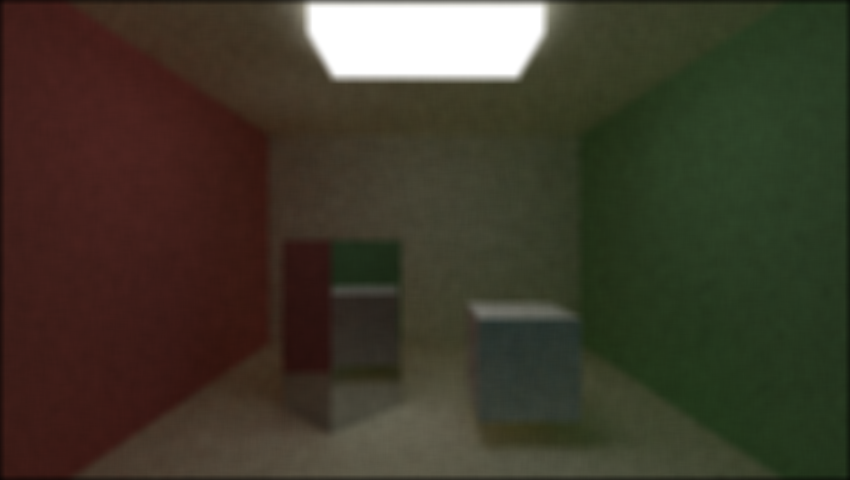
\includegraphics[scale=0.16]{media/mean/cornell_normal_50_mean_filter_11.png}
   	\end{figure}
   }
   { 
   \centering
   	\begin{figure}
   	\caption{Median Filter with window size $[11 \times 11]$.}  
   	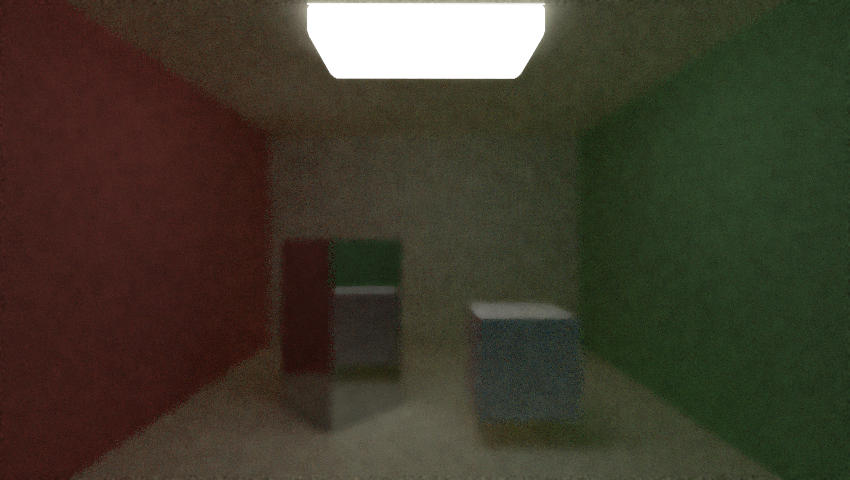
\includegraphics[scale=0.16]{media/median/cornell_normal_50_median_filter_11.png} 	
   	\end{figure}
   }
   {
   \centering
   	\begin{figure}
   	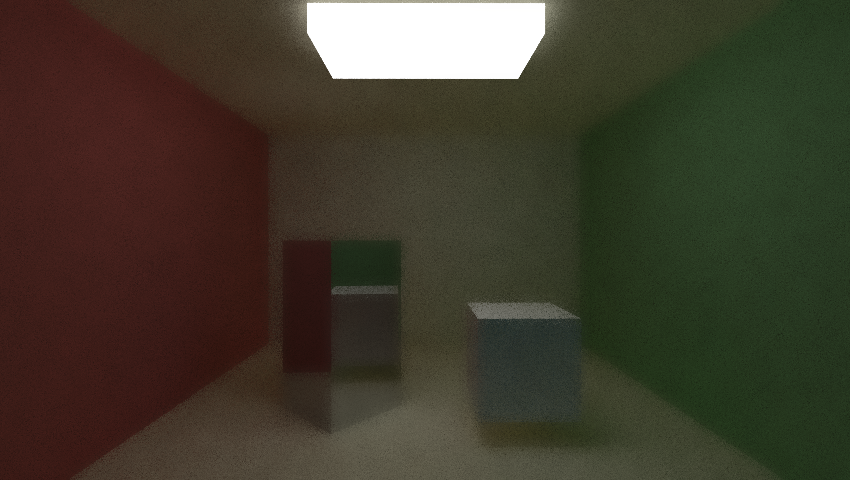
\includegraphics[scale=0.16]{media/bilateral/cornell_normal_50_bilateral_filter_21_15_10.png}
   	\caption{Bilateral Filter. Image with 50 SPP, $\delta_s = 15$ and $\delta_r = 10$}   	
   	\end{figure}
   }

\end{frame}


\begin{frame}%%     2
\begin{center}
{\fontsize{40}{50}\selectfont Thank you for your attention!}
\end{center}
\end{frame}


\end{document}
